%%%%%%%%%%%%%%%%%%%%%%% file template.tex %%%%%%%%%%%%%%%%%%%%%%%%%
%
% This is a general template file for the LaTeX package SVJour3
% for Springer journals.          Springer Heidelberg 2010/09/16
%
% Copy it to a new file with a new name and use it as the basis
% for your article. Delete % signs as needed.
%
% This template includes a few options for different layouts and
% content for various journals. Please consult a previous issue of
% your journal as needed.
%
%%%%%%%%%%%%%%%%%%%%%%%%%%%%%%%%%%%%%%%%%%%%%%%%%%%%%%%%%%%%%%%%%%%
%
% First comes an example EPS file -- just ignore it and
% proceed on the \documentclass line
% your LaTeX will extract the file if required
%\begin{filecontents*}{example.eps}
%!PS-Adobe-3.0 EPSF-3.0
%%BoundingBox: 19 19 221 221
%%CreationDate: Mon Sep 29 1997
%%Creator: programmed by hand (JK)
%%EndComments
%gsave
%newpath
%  20 20 moveto
%  20 220 lineto
%  220 220 lineto
%  220 20 lineto
%closepath
%2 setlinewidth
%gsave
%  .4 setgray fill
%grestore
%stroke
%grestore
%\end{filecontents*}
%
\RequirePackage{fix-cm}
%
%\documentclass{svjour3}                     % onecolumn (standard format)
%\documentclass[smallcondensed]{svjour3}     % onecolumn (ditto)
%\documentclass[smallextended]{svjour3}       % onecolumn (second format)
%\documentclass[twocolumn, referee]{svjour3}          % twocolumn
\documentclass[twocolumn, final]{svjour3}          % twocolumn % We Used!
%
\smartqed  % flush right qed marks, e.g. at end of proof
%
\usepackage{booktabs,caption,fixltx2e}
\usepackage[flushleft]{threeparttable}
\usepackage{graphicx}
\usepackage{helvet}         % selects Helvetica as sans-serif font
\usepackage{courier}        % selects Courier as typewriter font
\usepackage{type1cm}        % activate if the above 3 fonts are
\usepackage{bbding}
%\usepackage[ngerman,british]{babel}
%\usepackage{mathptmx}      % use Times fonts if available on your TeX system
\usepackage{float}
\usepackage{hyperref}
\usepackage[ddmmyyyy]{datetime}
\usepackage{latexsym}
\usepackage[misc]{ifsym}
%\usepackage{gensymb}
%\usepackage{algorithm}
\usepackage{makeidx}         % allows index generation
\usepackage[ruled]{algorithm2e} %ALgorithm
%\usepackage{algpseudocode}
\usepackage{pifont}
%\usepackage{multirow}
%\usepackage{multicol}        % used for the two-column index
%\usepackage[bottom]{footmisc}% places footnotes at page bottom
\usepackage{tcolorbox}
%\newtcbox{\hl}[1][yellow]{on line, arc=7pt,colback=#1!10!white,colframe=#1!50!black,
%  before upper={\rule[-3pt]{0pt}{10pt}},boxrule=1pt, boxsep=0pt,left=6pt,
%  right=6pt,top=2pt,bottom=2pt}
\usepackage{soul}		%Hughlighting package
%\useshorthands{"}
%\makeatletter
%\declare@shorthand{ngerman}{";}{\discretionary{-}{-}{-}\bbl@allowhyphens}
%\makeatother
%\addto\extrasbritish{\languageshorthands{ngerman}}

%%%%%%%%%%%
\usepackage{subcaption}

% ********************************** Tables ************************************
\usepackage{booktabs} % For professional looking tables
\usepackage{multirow}

%\usepackage{multicol}
%\usepackage{longtable}
%\usepackage{tabularx}


% ***************************** Math and SI Units ******************************

\usepackage{amsfonts}
\usepackage{amsmath}
\usepackage{amssymb}
\usepackage{siunitx} % use this package module for SI units

%%%%%%%%%%%
\usepackage{flexisym}
\usepackage{pdfpages}
\usepackage{epstopdf}
\usepackage{epsfig}

\usepackage{changepage}% http://ctan.org/pkg/changepage
\usepackage{lipsum}% http://ctan.org/pkg/lipsum

\usepackage{acronym}

\usepackage{tabulary}
\usepackage{tabularx}
\usepackage{makecell}
\usepackage{rotating}
% ******************************* Line Spacing *********************************

\usepackage{stackengine}
\usepackage{url}
\usepackage{cite}
\usepackage{balance}
%%%%%%%%%%%

\renewcommand{\dateseparator}{--}
% etc.
%
% please place your own definitions here and don't use \def but
% \newcommand{}{}
%
% Insert the name of "your journal" with
%\journalname{Cogn Comput (xxx) xx:xxx-xxx \\ DOI:10.1007/sxxxxx-xxx-xxxx-x}
\journalname{Cogn Comput}
\begin{document}

%\title{Insert your title here%\thanks{Grants or other notes
%about the article that should go on the front page should be
%placed here. General acknowledgments should be placed at the end of the article.}
%}
%\subtitle{Do you have a subtitle?\\ If so, write it here}

%\titlerunning{Short form of title}        % if too long for running head

%\author{First Author         \and
%        Second Author %etc.
%}

%\title{A Neuro-Fuzzy based Control System for Solar Powered Wheelchair based on Feature Extraction of Surface Electromyogram Signal}
\title{A Gaussian Process Model for Inferring the Dynamic Transcription Factor Activity using Ornstein-Uhlenbeck Kernel}
\titlerunning{GP model for Inferring TFA}
% Use \titlerunning{Short Title} for an abbreviated version of
% your contribution title if the original one is too long
\author{Muhammad Arifur Rahman
    \and Neil D. Lawrence}

\authorrunning{M A Rahman et al.}

%\authorrunning{Neuro-Fuzzy based Solar Powered Wheel Chair Control using sEMG signal}
% Use \authorrunning{Short Title} for an abbreviated version of
% your contribution title if the original one is too long
\institute{
    Muhammad Arifur Rahman (\Letter)
        \at Department of Computer Science, University of Sheffield, UK
        \at Department of Physics, Jahangirnagar University, Savar, 1342 - Dhaka, Bangladesh 
        \at \email{arif@juniv.edu}
    \and Neil D Lawrence %(\Letter)
        \at Department of Computer Science, University of Sheffield, UK  
        \at Amazon, UK.
        %\email{N.Lawrence@sheffield.ac.uk}
        }

\date{Received: \today / Accepted: date}
% The correct dates will be entered by the editor


\maketitle

\abstract{ In molecular biology and genetics, a transcription factor is a protein that binds to specific DNA sequence. Transcription factors control the flow (or transcription) of genetic information from DNA to mRNA. To develop models of cellular processes quantitative estimation of the regulatory relationship between transcription factors and genes is an essential requirement. While modelling transcription factor activity, a Markovian assumption based state space model where any state solely depends on its previous state might not be a suitable option as a general case. The Gaussian process, a nonparametric model, can easily overcome this state dependency. However, designing a covariance function for Gaussian process model is crucial. In this paper, we justified the rationale for the choice of the Ornstein-Uhlenbeck covariance function and developed a Gaussian process model to figure out the dynamics of transcription factor activity. 
}

 \section{Introduction}
%\subsection{Motivation behind the study of TFA}\label{sec:TFA_Motovation} 
In the consequences of diverse internal and external stimuli, cellular life must recognise and respond appropriately. Gene expression is the converted form of an abstract code of biological information preserved inside the DNA. Gene expression is a tightly regulated process which allows cells to respond to any internal and external stimuli or change of environment. With very few minor exceptions, all cell types in a multicellular organism preserve the identical genetic information. For a specified organism, any individual cell type expresses only a unique subset of the total number of distinct genes. Differentially expressed genes are specified by unique epigenetic information. This information is present in the distinct cell and also determines the phenotype of the composite organism \cite{Keller:1994, Alberts:2002}. 

DNA transcription is a process that controls the first step of gene expression and transcribes genetic information from DNA to RNA. The transcription process is pivotal to produce proteins, and the transcription profile is a highly preferable parameter for the recognition of a distinct cell type. In general, a complex biological regulatory network controls the differential gene expression, in which particular transcription factors relay the signals to specific target genes. Among these transcription factors, many of them are DNA-binding proteins, which bind to regulatory DNA elements located cis to the target genes \cite{Calkhoven:1996}.

Using microarray experiments systematic gene expression quantification has been introduced decades ago \cite{Schena:1995} yet the recent development of chromatin immunoprecipitation (ChIP) followed by microarray (also known as ChIP-chip) and sequencing (also known as ChIP-seq) technologies boosted the genome-wide identification of transcription factor \cite{Ren:2000, Horak:2002}.

Transcription factors (TFs) are expository for the transcriptional regulation and the transcriptional regulatory system plays a pivotal role in controlling many biological processes, ranging from cell cycle progression and preservation of intracellular metabolic and physiological stability \cite{Simon:2001, Takahashi:2006}. It also plays a crucial role in cellular differentiation and developmental dynamics by ensuring the meticulous expression of specific genes \cite{Dynlacht:1997}. There are two types of Transcription factors: some of them are \emph{general} and rest are \emph{sequence-specific}. \emph{General} transcription factors act collaboratively with RNA polymerase II and are ubiquitously involved in the transcription of a large number of genes \cite{Lee:2000}. \emph{Sequence-specific} transcription factors bind particular subsets of target genes, leading to well defined spatio-temporal patterns of gene expression \cite{Kadonaga:2004}.

A number of diseases emerge from a breakdown in the regulatory system: transcription factors are over-represented among oncogenes \cite{Furney:2006}, and almost one-third of human developmental disorders have been ascribed to dysfunctional TFs \cite{Boyadjiev:2000}. Even alterations in the activity and regulatory specificity of transcription factors are likely to be a primary reason for evolutionary adaptation and phenotypic diversity \cite{Subhajyoti:2008}. Indeed, recent research and study have already proved that increased sophistication of the transcriptional regulatory system seems to have been a key requirement for the emergence of metazoan life \cite{Levine:2003}. So inferring the dynamics of transcription factors activities might play a significant role to obtain a deeper insight into the gene regulatory network.

To build a transcriptional regulatory network, it may appear that knowledge of particular biomedical functions of transcription factors are not important. Even with some naive assumptions, it may appear that promoters or repressors regulate the transcription process similarly under similar condition. However, these assumptions can't be considered as general rules as it already reported that transcription factor DNA binding events might not follow the exact or defined biological regulatory mechanism. Such as, in a study, \cite{Turcotte:1992} reported that in different mutants of yeast \emph{HAP1} positive control could selectively affect different gene expressions. Using comparative genomics and functional scanning of transgenic mice \cite{Menke:2008} showed how the transcription factor \emph{TBX4} plays a pivotal role in hindlimb and vascular development. They showed a group of enhancers control the gene expresses level in different tissues. Genomic analysis also showed the relationship between transcription factor binding events and transcription factors from genes affected by the mutation. In their study \cite{Hughes:2013} explained even further where they reported about the role of cofactors during the transcriptional mechanism. Only understanding of condition-specific activation, noise presence in the data or transcriptional cascades is not enough to grasp the actual understanding of these phenomena. Therefore, to dissect the regulatory mechanisms and gaining a better insight the complete index of transcription factor activities and its interacting partners would be invaluable.

%%%%% Added
Modelling transcription factor activities can be seen as latent variable modelling \cite{Bishop:1999, Lawrence:2005}. We can observe the gene expression level, but these expression levels are regulated by protein-coding genes that bind to a specific DNA sequence and controls the production rate of mRNA. These gene expression levels are analogous to the movement of the marionette (Figure \ref{fig:LVM_Cartoon}), but the transcription factor's activity is unobservable like the puppeteer's control bar which controls the gene expression levels.
\begin{figure}
	\centering
	%\includegraphics[width=0.7\textwidth,keepaspectratio]{LVM_Cartoon.png}
		\includegraphics[width=0.45\textwidth,keepaspectratio]{diagrams/LVM_Cartoon.png}
	\rule{25em}{0.5pt}
	\caption[Marionette analogy of latent variable model]
	{Marionette analogy of latent variable model: Marionette's different dynamics are observed (later represented by $\textbf{Y}$ in the Section \ref{sec:Probabilistic_TFA}). But these movements are controlled by the puppeteer's control bar which is unobserved (later these dynamics represented by $\textbf{X}$ in the Section \ref{sec:Probabilistic_TFA}).}
	\label{fig:LVM_Cartoon}
\end{figure}

In recent years an idea that has gained a lot of interest to infer the regulatory mechanism from the expression levels of genes. There has been a wealth of research on microarray data. A number of methods \cite{Alter:2004, Gao:2004, Liao:2003} aim to infer a matrix of transcription factor activities (TFAs). These TFAs can be summed up in a single number at a certain experimental point to find the concentration of the transcription factor and its binding affinity to its target genes. A variety of approaches has been proposed to infer these TFAs. For example, \cite{Liao:2003} developed a data decomposition technique with dimension reduction and introduced the concept of ‘network component analysis’. This method takes account of the connectivity information by imposing algebraic constraints on the factors. They argued that classical statistical methods such as principal component analysis and independent component analysis, do not consider the underlying network structure while computing low dimensional or hidden representation of a high-dimensional data sets like DNA microarray. 

Later \cite{Alter:2004} used a dimension reduction technique (singular value decomposition) to figure out TFAs and also the correlation between DNA replication initiation and RNA transcription during the yeast cell cycle. Using multivariate regression and backward variable selection to identify active transcription factors \cite{Gao:2004} targeted the same; \cite{Boulesteix:2005} used the partial least squares (PLS) regression to infer the true TFAs from a combination of tRNA expression and DNA-protein binding measurement. A major drawback of the methods mentioned above is that transcription factor activities do not hold any information regarding the strength of the regulators' interactivity between the transcription factors and its different target genes. It is expected that depending on the experimental conditions the transcription factor activities can vary from gene to gene. It is also expected that different transcription factors may bind to the same gene. In most cases, realistic information about the intervals may not be true as they were not based on the fully probabilistic model. Moreover, false positives are always a problem for connectivity data, typically a significant portion of ChIP data suffers from it \cite{Boulesteix:2005}. Furthermore, due to the various cellular process or changes in environmental conditions the structure of the regulatory network of the cell can change considerably. Using regression-based methods, it is difficult to track these changes. \cite{Nachman:2004} built a probabilistic model, using the basic framework of dynamic Bayesian networks based on discrete random variables for protein concentrations and binding affinities. Though the model was more realistic, the computational complexity for genome-wide analysis can be expensive.
%%%%%

Here in this paper, we model a kernel or covariance function of the Gaussian process for reconstructing transcription factor activities where the gene expression profiles and the connectivity information of binding data (connectivity matrix) between genes and transcription factors are given. Our modelling framework initiated from the ideas of \cite{Sanguinetti:2006} where they used a linear-Gaussian state-space modelling framework to infer the TFA. 

We note that the TFA model proposed by \cite{Sanguinetti:2006} is a linear Gaussian state space model with Markov property. A model with Markov property have the state dependencies; i.e. any certain state depends on the transition probability of previous state (or states for order-$k$ Markov model).  This state dependency with Markov property may deem as a restrictive assumption where the transition probability from the first state to the second state is completely different from the transition from the second state to the third state and so on.  We also noticed that the linear Gaussian state space model of TFA proposed by \cite{Sanguinetti:2006} is identical to a Gaussian process model with a particular kernel or covariance function. In general, this kernel or covariance function of a Gaussian process is constructed considering the similarity measure between every possible input pairs (or states). We, therefore, started our modelling framework directly from the Gaussian process perspective to attain the same target. We also propose a computational trick, based on  judicious application of singular value decomposition (SVD), to fit the Gaussian process efficiently in a reduced \lq transcription factor activity\rq{ }space. 

In the probabilistic inference of TFAs, \cite{Spellman:1998} used gene expression time series of synchronized yeast cells from the cell division cycle gene CDC-15 (Systematic name YAR019C) experiment. 
The second data set is from ChiP-chip \cite{Ren:2000, Horak:2002} experiments performed on yeast by \cite{Lee:2002}. We constructed the binding information between transcription factors and genes. In this paper we are going to combine this binding information with the gene expression information to infer transcription factor activities.

\section{Gaussian Process}
A Gaussian process (GP) is a collection of random variables, any finite number of which have a joint Gaussian distribution \cite{Rasmussen_and_Williams:2006}. It is a continuous stochastic process and defines probability distributions for functions. It can be also viewed as a collection of random variables indexed by a continuous variable. Any finite set of values from the collection can be written as a vector. Let's consider $ \textbf{f} = \{ f_1, f_2, f_3,..., f_N\}$ corresponds with indexed inputs $ \textbf{X} = \{ \textbf{x}_1, \textbf{x}_2, \textbf{x}_3,..., \textbf{x}_N\}$. In Gaussian processes, variables from these random functions are jointly normally distributed and as a whole can be represented as a multivariate Gaussian distribution
\begin{equation} \label{eq:2.2}
p(\textbf{f}|\textbf{X})\sim \mathcal{N}\left(\textbf{f}|\boldsymbol\mu,\textbf{K}\right),
\end{equation}
where $\boldsymbol\mu$ is the mean and $\textbf{K}$ is the covariance matrix. Both potentially depends on $\textbf{X}$. The Gaussian distribution is over vectors but the Gaussian process is over functions.

We need to define the mean function and covariance function for a Gaussian process prior. If $f(\textbf{x})$ is a real valued process, a Gaussian process is completely defined by its mean function and covariance function given in Equation \ref{eq:2.3} and Equation \ref{eq:2.4} respectively. Usually the mean function $m(\textbf{x})$  and the covariance function $k(\textbf{x},\textbf{x\textprime})$ are defined as
\begin{equation} \label{eq:2.3}
m(\textbf{x})= \mathbb{E}[f(\textbf{x})],
\end{equation}
and
\begin{equation} \label{eq:2.4}
k(\textbf{x},\textbf{x\textprime})= 
\mathbb{E}[(f(\textbf{x})-m(\textbf{x}))(f(\textbf{x}\textprime)-m(\textbf{x}\textprime))],
\end{equation}
where $\mathbb{E}$ represents the expected value. We denote the Gaussian process as
\begin{equation} \label{eq:GP}
f\left(\textbf{x} \right)\sim \mathcal{GP} \left(m \left(\textbf{x}\right), k \left(\textbf{x},\textbf{x\textprime}\right) \right).
\end{equation}
The covariance matrix $\textbf{K}$ is constructed from the covariance function $k(\textbf{x},\textbf{x\textprime})$ and $\textbf{K}_{ij}=k\left(\textbf{x}_i,\textbf{x}_j\right)$, that is 
\begin{equation} \label{eq:GP_cov_mat}
\textbf{K} = 
\begin{pmatrix}
k\left(\textbf{x}_1,\textbf{x}_1\right) & k\left(\textbf{x}_1,\textbf{x}_2\right) & \cdots & k\left(\textbf{x}_1,\textbf{x}_n\right) \\
k\left(\textbf{x}_2,\textbf{x}_1\right) & k\left(\textbf{x}_2,\textbf{x}_2\right) & \cdots & k\left(\textbf{x}_2,\textbf{x}_n\right) \\
\vdots  & \vdots  & \ddots & \vdots  \\
k\left(\textbf{x}_n,\textbf{x}_1\right) & k\left(\textbf{x}_n,\textbf{x}_2\right) & \cdots & k\left(\textbf{x}_n,\textbf{x}_n\right)
\end{pmatrix}.
\end{equation}
Loosely speaking, a Gaussian process is multivariate Gaussian distribution defined over an infinite number of dimensions. A sample from a Gaussian process is a random function. While a $n-$dimensional Gaussian distribution is fully specified by mean $\boldsymbol\mu$, a $n \times 1$ vector of expectations and covariance matrix $\textbf{K}$, the $n \times n$ matrix of covariances between all pair of points.

It is a common practice to consider a Gaussian process with zero mean when no prior information is available. This is not excessively restrictive as a variety of functions can be generated by a zero mean process. A second order stationary process has a constant mean and the covariance function solely depends on the distance between the inputs. Zero-mean process is a simplification just by centring the data as $\textbf{t} = \textbf{t} - \overline{\textbf{t}}$, where $\overline{\textbf{t}}$ is the data sample mean. An extra constant term with the covariance function can reflect the variation from the mean of the process \cite{MacKay:2003}. So, a constant-mean or a zero-mean assumption is not overly restrictive in practice.

\subsection{GP: Covariance Functions}
The covariance function (also called kernel, kernel function or covariance kernel) characterises the properties or nature of the samples drawn from a Gaussian process. The covariance function encodes the modelling assumptions we wish to incorporate in our application. The mandatory requirement of a covariance matrix is to be symmetric positive semi-definite\footnote{A matrix $\textbf{C}$ is called positive semi-definite if $\textbf{z}^{\top}\textbf{C}\textbf{z} \geq 0$ for all $\textbf{z}$. Where $\textbf{z}$ is a non zero column vector of length $n$, $\textbf{C}$ is a $n\times n$ symmetric real matrix and $\textbf{z}^{\top}$ is the transpose of $\textbf{z}$.}. So, as long as the covariance function generates symmetric positive semi-definite matrix, we can use that function for a Gaussian process. Smoothness, periodicity, amplitude, lengthscale etc. are basic properties that can be incorporated while designing Gaussian process covariance function. Once the decision to model with a Gaussian process has been made the choice of the covariance function is a central step in modelling. The main goal of this thesis is to develop covariance functions suitable for transcription factor activity analysis and clustering gene expressions. Here we will discuss some of the very well known and widely used covariance functions. A wide choice of valid covariance functions and their detail description can be found in \cite{Rasmussen_and_Williams:2006}.

Any form of covariance function is acceptable, provided it satisfies the following equation
\begin{equation} \label{eq:cov_basic}
\sum_{i,j} a_i a_j k\left(\textbf{x}_i,\textbf{x}_j\right)\geq 0
\end{equation}
where, $a_i, a_j \dots a_n$ are arbitrary real coefficients and $\textbf{x}_i, \textbf{x}_j \dots \textbf{x}_n$ are finite set of data points. A covariance function is termed \lq stationary\rq when it follows
\begin{equation} \label{eq:cov_stationary}
\text{Cov}\left[f\left(\textbf{x}_i\right),f\left(\textbf{x}_j\right)\right] = k\left( \lVert \textbf{x}_i -\textbf{x}_j \rVert \right)
\end{equation}
for all $\textbf{x}_i,\textbf{x}_j \in \mathbb{R}^D$. In practice, a stationary covariance function gives a function that is invariant to translation and does not depend on the absolute location of the corresponding inputs; rather it depends on the distance separating them. 

If the covariance does not only depend on the distance between the data points in the input space, rather the model needs to adapt to functions where smoothness varies with the inputs, a non-stationary covariance function will be required. There are many interesting non-stationary covariance functions. Depending on the nature or trend a careful selection of appropriate covariance function is essential. One of the simplest examples of non-stationary covariance function which have a linear trend can be expressed by 
\begin{equation} \label{eq:cov_nonStationary}
k\left( \textbf{x}_i, \textbf{x}_j \right) = \sum_{d=1}^{D} a_d x_i^d x_j^d
\end{equation}
where $x_i^d$ is the $d^{th}$ component of $\textbf{x}_i \in \mathbb{R}^D$. 

In this paper, as a prior, we used some stationary covariance functions and in the following section, we briefly describe some of them. Non-stationary covariance functions are beyond our scope and a detailed description is available in \cite{Rasmussen_and_Williams:2006}.

\subsection{The Mat{\'e}rn Covariance Function}
The Mat{\'e}rn class of covariance functions can be expresses by Equation \ref{eq:Matern_cov}
\begin{equation} \label{eq:Matern_cov}
K_{Mat}(r)= a^2\frac{2^{1-\nu}}{\Gamma(\nu)}\left(\frac{\sqrt{2\nu}r}{l}\right)^\nu K_{\nu}
\left(\frac{\sqrt{2\nu}r}{l}\right)
\end{equation}
where $a, l, \nu$ are positive hyperparameters, $K_{\nu}$ is a modified Bessel function and $\Gamma \left(.\right)$ is the Gamma function. Hyperparameter $\nu$ controls the roughness of the function and like Exponentiated quadratic covariance function the parameters $a$ and $l$ controls the amplitude and lengthscale respectively. Though for $\nu \to \infty$ we can obtain the exponentiated quadratic kernel. For finite value of $\nu$, the sample functions are significantly rough. 

The simpler form of Mat{\'e}rn covariance function is obtained when $\nu$ is considered as a  half-integer: $\nu = p+1/2$, where $p$ is a non-negative integer. The covariance function can be expressed as a product of an exponential and a polynomial of order $p$. In \cite{Abramowitz:1965} Abramowitz et al. derived the general expression as follows
\begin{equation} \label{eq:MaternGeneral}
\begin{split}
K_{\nu=p+1/2}(r)&= a^2\exp \left( - \frac{\sqrt{2\nu}r}{l}\right)\frac{\Gamma\left(p+1\right)}{\Gamma\left(2p+1\right)}\\
&\sum_{i=0}^{p}\frac{\left(p+i\right)!}{i!\left(p-i\right)!}
\left(\frac{\sqrt{8\nu}r}{l}\right)^{p-i}.
\end{split}
\end{equation}
The most interesting cases for machine learning are $\nu =3/2$ and $\nu=5/2$, for which we get the following equations respectively
\begin{equation} \label{eq:Matern32}
K_{\nu=3/2}(r)= a^2 \left(1+ \frac{\sqrt{3}r}{l} \right)\exp \left( - \frac{\sqrt{3}r}{l} \right)
\end{equation}
and
\begin{equation} \label{eq:Matern52}
K_{\nu=5/2}(r)= a^2 \left(1+ \frac{\sqrt{5}r}{l} + \frac{5r^2}{3l^2} \right)
\exp \left( - \frac{\sqrt{5}r}{l} \right).
\end{equation}

\begin{figure}[!htbp]
	\centering
	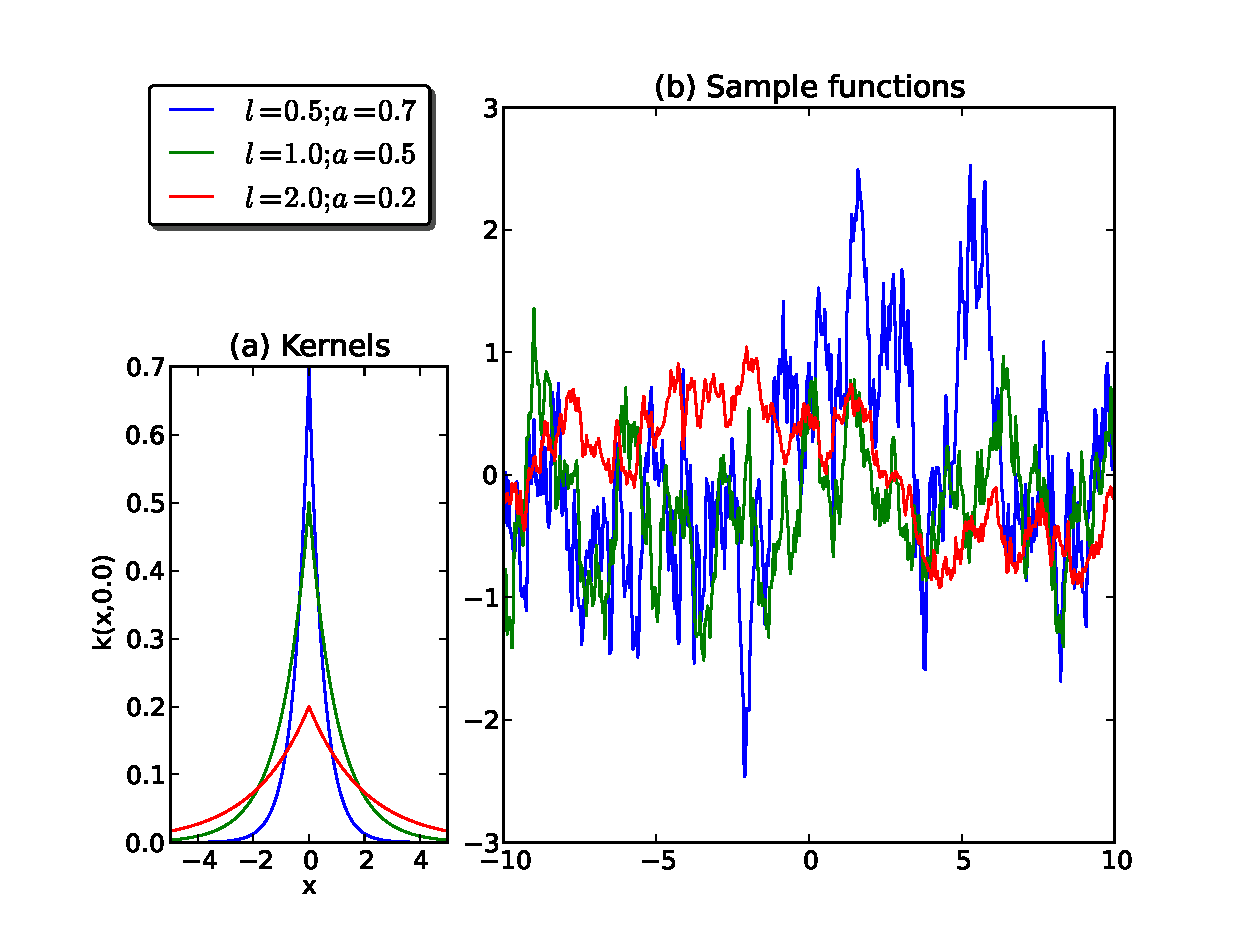
\includegraphics[width=0.5\textwidth,keepaspectratio]{diagrams/OU_cov.eps}
	\rule{25em}{0.5pt}
	\caption[The OU kernels and random sample functions]
	{The OU kernels (a) and random sample functions (b) for different hyperparameter settings shown in the top left.}
	\label{fig:OU_covariance}
\end{figure}

\subsection{The Ornstein-Uhlenbeck Process}
The Ornstein-Uhlenbeck process \cite{Ornstein_Uhlenbeck:1930} is a special case of Mat{\'e}rn class covariance functions. The Ornstein-Uhlenbeck (OU) process was developed as a mathematical model of the velocity of a particle moving with Brownian motion.

The Ornstein-Uhlenbeck process can be found setting up $\nu=1/2$ and expressed as Equation \ref{eq:OU}. Figure \ref{fig:OU_covariance}$(a)$ shows the kernel and Figure \ref{fig:OU_covariance}$(b)$ shows the sample functions form the OU process  with different hyperparameter settings as shown to the left of the figure.  
\begin{equation} \label{eq:OU}
K_{\nu=1/2}(r)= a^2 \exp \left(-\frac{r}{l} \right)
\end{equation}


\begin{figure*}[!htbp]
	\centering
	\includegraphics[width=\textwidth,keepaspectratio]{diagrams/ConstructKernels_BR_Cos.pdf}
	\rule{45em}{0.5pt}
	\caption[Construction of a new kernel adding two basic kernels]
	{Construction of \lq made by order\rq kernel adding two basic kernels: an example of a univariate data which is globally periodic and locally governed by some random motions. (top-left) a sample taken using Brownian kernel, (top-middle) a sample is taken using Cosine kernel, (top-right) a sample taken using a newly constructed kernel by adding two kernels, (bottom-left) Brownian kernel, (bottom-middle) Cosine kernel, (bottom-right) newly constructed kernel.} 
	\label{fig:ConstructKernels_BR_Cos}
\end{figure*}

\subsection{Constructing Kernels}

Modelling kernel is the central step in Gaussian process modelling. A number of \lq built-in\rq{ }kernels (both stationary and non-stationary) are available for Gaussian process, yet we may need to model a complicated structure which is not expressed very well by any known kernel. To model such a structure, we may build our own \lq customised kernel\rq{ }with the required structure or, desired properties. An addition of two Gaussian variables is a Gaussian. Scaling a Gaussian also leads to a Gaussian. These two basic mathematical properties help to develop a range of kernels from a very simple one to complex a one. 

Assume an univariate data is globally periodic and local structures governed by some random motions (Brownian motion). There are multiple choices dealing with the global structure and one of the possible solutions could be a Cosine kernel for the global structure and a Brownian kernel for local structures in an additive form. The addition of two positive semi-definite kernels together always results in another positive semi-definite kernel. Figure \ref{fig:ConstructKernels_BR_Cos} shows the sample functions and representation of the newly constructed kernel.

\subsection{Gaussian Process Regression}
Gaussian process regression can be done using the marginal and conditional properties of the multivariate Gaussian distribution. Let's consider that we have the observation $\mathbf{f}$ of a function at the observation point $\mathbf{x}$. Now we wish to predict the values of that function at the observation points $\mathbf{x_\star}$, which are represented by $\mathbf{f_\star}$. Then the joint probability of $\mathbf{f}$ and $\mathbf{f_\star}$ can be obtained as 
\begin{equation} \label{eq:jointPro_f_f*}
p \left( \begin{bmatrix} \mathbf{f} \\\mathbf{f_\star} \end{bmatrix} \right) =
\mathcal{N}\left( \begin{bmatrix} \mathbf{f} \\\mathbf{f_\star} \end{bmatrix} \middle|
\mathbf{0}, \begin{bmatrix} \mathbf{K_{x,x}} & \mathbf{K_{x,x_\star}} \\
\mathbf{K_{x_\star,x}} & \mathbf{K_{x_\star,x_\star}} \end{bmatrix} \right)
\end{equation}
where the covariance matrix $ \mathbf{K_{x,x}}$ has elements derived from the covariance function $ k \left(x,x\textprime \right)$, such that the $ \left(i,j \right)^{th}$ element of $\mathbf{K_{x,x}}$ is given by $k \left( \mathbf{x} \left[ i\right],\mathbf{x} \left[ i\right] \right)$. The conditional property of a multivariate Gaussian is used to perform regression. The conditional property can be represented by

\begin{equation} \label{eq:condProMvG}
p \left( \mathbf{f_\star} \middle| \mathbf{f} \right) =
\mathcal{N}\left( \mathbf{f_\star} \middle| \mathbf{K_{x_\star,x}}  \mathbf{K^{-1}_{x,x}} \mathbf{f,} \mathbf{K_{x_\star,x_\star}} - 
\mathbf{K_{x_\star,x}} \mathbf{K^{-1}_{x,x}} \mathbf{K_{x,x_\star}}\right).
\end{equation}

In an ideal case, the observation $\mathbf{f}$ is noise-free, but, in practice, it is always corrupted with some noise. Let's consider $\mathbf{y}$ as a corrupted version of $\mathbf{f}$. If we consider this noise as Gaussian noise, we can write $p \left( \mathbf{y} \middle| \mathbf{f} \right) = \mathcal{N} \left( \mathbf{y} \middle| \mathbf{f}, \sigma^2 \mathbf{I} \right) $, where $ \sigma^2 $ is the variance of the noise and $\mathbf{I}$ is the identity matrix with the appropriate size and marginalise the observation $\mathbf{f}$. Then, the joint probability of $\mathbf{y}$ and $\mathbf{f_\star}$ can be represented by 

\begin{equation} \label{eq:jointPro_y_f*}
p \left( \begin{bmatrix} \mathbf{y} \\\mathbf{f_\star} \end{bmatrix} \right) =
\mathcal{N}\left( \begin{bmatrix} \mathbf{y} \\\mathbf{f_\star} \end{bmatrix} \middle|
\mathbf{0}, \begin{bmatrix} \mathbf{K_{x,x}}+ \sigma^2\mathbf{I} & \mathbf{K_{x,x_\star}} \\
\mathbf{K_{x_\star,x}} & \mathbf{K_{x_\star,x_\star}} \end{bmatrix} \right).
\end{equation}

Regression with Gaussian process is a Bayesian method. From the knowledge of a \emph{prior} over a function and data, we infer a \emph{posterior} and this happens in a closed form of Equation \ref{eq:condProMvG}. 

\begin{figure}[!htbp]
	\centering
	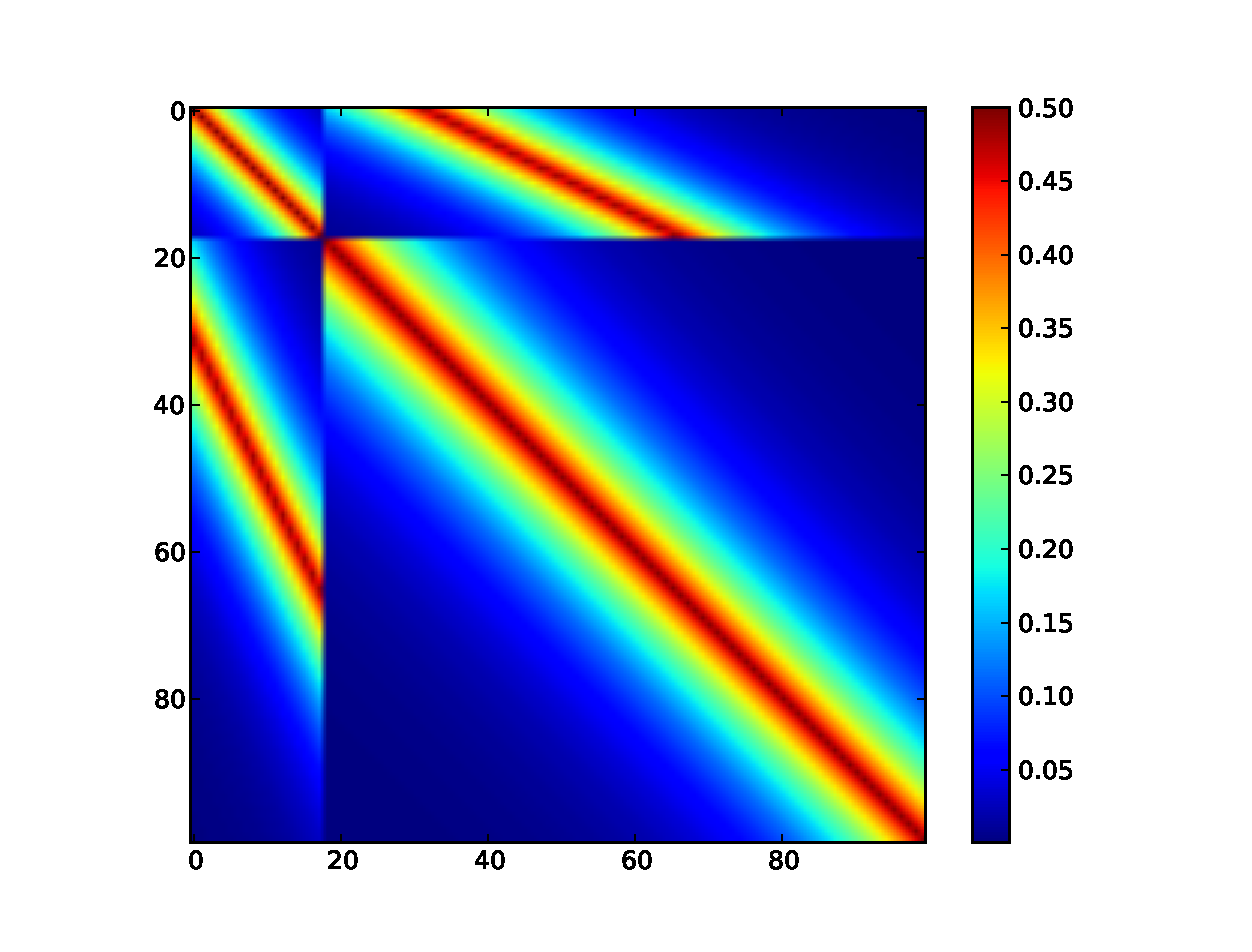
\includegraphics[width=0.5\textwidth,keepaspectratio]{diagrams/Cov_Structure.eps}
	\rule{25em}{0.5pt}
	\caption[Overall representation of covariances between training and test data]
	{Overall representation of covariances between training and test data.}
	\label{fig:Covariances_Structure}
\end{figure}

Figure \ref{fig:Covariances_Structure} shows the overall covariance structure between some training and test data. For this example, we choose 18 training points and 82 test points. We observe the shaded structure because some of the training data are closer to some of the test data. Observing this structure, we can also figure out the closeness between training and test data. 


\subsection{Making Predictions}
The probability density is represented by functions. Due to consistency this density is known as a process. Also by this property, any future values of $\mathbf{f_\star}$ which are unobserved can be predicted without affecting $\mathbf{f}$. To make predictions of the test data, we use the conditional distribution. In an ideal case, the conditional distribution is $p\left(\mathbf{f_\star}\middle| \mathbf{f} \right)$ and if we consider the noise, the conditional distribution will be $ p\left( \mathbf{f_\star} \middle| \mathbf{y} \right) $. Both of the distributions are also Gaussian
\begin{equation} \label{eq:prediction}
\mathbf{f_\star}  \sim \mathcal{N} \left( \boldsymbol{\mu}_f, \mathbf{C}_f \right).
\end{equation}
The mean of the conditional distribution in Equation \ref{eq:prediction} is
\begin{equation} \label{eq:prediction_mean}
\boldsymbol{\mu}_f = \mathbf{K_{x,x_\star}^\top} \left[ \mathbf{K_{x,x}}+ \sigma^2\mathbf{I} \right]^{-1} \mathbf{y}
\end{equation}
and its covariance is given by
\begin{equation} \label{eq:prediction_cov}
\mathbf{C}_f = \mathbf{K_{x_\star,x_\star}} -
\mathbf{K_{x,x_\star}^\top} \left[ \mathbf{K_{x,x}}+ \sigma^2\mathbf{I} \right]^{-1} \mathbf{K_{x,x_\star}}.
\end{equation}

\begin{figure}
	\centering
	\includegraphics[width=0.5\textwidth]{diagrams/gpreg.pdf}
	\rule{25em}{0.5pt}
	\caption[A representation of Gaussian process regression: Modelling one-dimensional function using Gaussian process]
	{A representation of Gaussian process regression: Modelling one-dimensional function using Gaussian process. Coloured solid lines represent different samples from the process and the dotted line is the mean function. The shaded area is the 95\% confidence interval. (a) A Gaussian process not conditioned on any data points. Without any observations, the prior uncertainty about the underlying function is constant everywhere. (b-e) The posterior after conditioning on different amount of data.}
	\label{fig:dempGPReg}
\end{figure}

These results can be calculated using the block matrix inverse rules. Figure \ref{fig:dempGPReg} shows a visual representation of Gaussian process regression for a one-dimensional function. Coloured solid lines represent different samples from the process and the dotted line is the mean function. The shaded area is the 95\% confidence interval. Figure \ref{fig:dempGPReg}(a) represents a Gaussian process not conditioned on any data points. Without any observations, the prior uncertainty about the underlying function is constant everywhere. Figure \ref{fig:dempGPReg}(b-e) show some posterior samples after conditioning on different amount of training data as shown in the figure. 

\subsection{Hyperparameter Learning}
To construct the covariance function, still we need to consider the hyperparameters and optimize them. These adjustable parameters alter the distribution of the function output values obtained from a Gaussian process. The most efficient and commonly used optimization technique for hyperparameters is maximum likelihood. If we consider all the hyperparameters $\alpha$ (controls the amplitude), $\sigma^2$ (variance of the noise) and $l$ (length-scale) in a vector $\boldsymbol{\theta}$, we can use gradient methods to optimize $p \left(\mathbf{y}\middle|\boldsymbol{\theta}\right)$ with respect to $\boldsymbol{\theta}$. The Log likelihood is given by

\begin{equation} \label{eq:Likelihood}
\begin{split}
\text{log } p\left(\mathbf{y}\middle|\boldsymbol{\theta}\right) &=
- \frac{D}{2}\text{log}2\pi - \frac{1}{2}\times \text{log} \left| \mathbf{K_{x,x}} + \sigma^2\mathbf{I}\right|\\
&- \frac{1}{2}\mathbf{y}^\top \left[\mathbf{K_{x,x}} + \sigma^2\mathbf{I} \right]^{-1}\mathbf{y}.
\end{split}
\end{equation}

We can have the log maximum likelihood by
\begin{equation} \label{eq:LML}
\boldsymbol{\theta}_{max} =  \operatorname*{arg\,max}_\theta \left( p\left(\mathbf{y}\middle|\boldsymbol{\theta}\right) \right).
\end{equation}

%%%%
\section{Mechanistic model of TFA}\label{sec:Probabilistic_TFA}
The logged gene expression measurements are collected in a design matrix, $\textbf{Y} \in \mathbb{R}^{ N \times d}$ where $N$ is the number of genes and $d$ is the time points or number of experiments. The binary matrix $\textbf{X} \in \mathbb{R} ^ {N \times q}$ is the connectivity measurements, where $q$ is the number of transcription factors. We assume that $\textbf{X}_{i,j}$ is \lq 1\rq{ }if transcription factor $j$ can bind gene $i$, \lq 0\rq{ }otherwise.

In \cite{Sanguinetti:2006} Sanguinetti et al. used a latent variable model. TFAs were obtained by regression from the gene expressions using the connectivity information, given the following linear model 
\begin{equation} \label{eq:linear_model_TFA}
\textbf{y}_n = \textbf{B}_n \textbf{x}_n + \boldsymbol{\epsilon_{n}}
\end{equation}
Here $n = 1, . . . ,N$ indexes the gene, $\textbf{y}_n =\textbf{Y}(n,:)^{\top}$, $\textbf{x}_n=\textbf{X}(n,:)^{\top}$ and $\boldsymbol{\epsilon_{n}}$ is an error term. The matrix $\textbf{B}_n$ has $d$ rows and $q$ columns, and models the gene specific TFAs.

Different TFAs for every individual gene will increase number of model parameters drastically. This huge parameter space can be dealt through marginalization by prior distribution on the rows of $\textbf{B}_n$. Yet, 
two physically plausible assumptions for selecting the prior distribution will be helpful to determine the gene specific TFAs. 
\begin{itemize}
	\item The first assumption: $\textbf{b}_{nt}$ has the Markov property and hence gene specific TFA $\textbf{b}_{nt} $ at time $t$ depends exclusively on the gene specific TFA at time $(t-1)$.
	\item The second assumption: the prior distribution to be stationary in time.
\end{itemize}

In order to support these assumptions, there will be two limiting cases for prior distributions. Let's first assume all the $\textbf{b}_{nt}$ are identical for all $t$. Then the first limiting case is
\begin{equation} \label{eq:limit_one_a}
\textbf{b}_{n1} \sim \mathcal{N} ( \boldsymbol{\mu},\boldsymbol{\Sigma}), 
\end{equation}
and
\begin{equation} \label{eq:limit_one_b}
\textbf{b}_{n(t+1)} \sim \mathcal{N} ( \textbf{b}_{nt},\textbf{0}).
\end{equation}
If the experimental dataset comes by replicating a condition then this model is an appropriate one. The second limiting case appears when all the $\textbf{b}_{nt}$ are independent and identically distributed (iid)
\begin{equation} \label{eq:limit_two}
\textbf{b}_{nt}\sim \mathcal{N} ( \boldsymbol{\mu},\boldsymbol{\Sigma}).
\end{equation}
This is the case when experimental dataset comes from independent samples drawn without any temporal order.

Sanguinetti et al. \cite{Sanguinetti:2006} expected a realistic model of time series data to be somewhere in between these two extremes (Equation \ref{eq:limit_one_a}, Equation \ref{eq:limit_one_b} and Equation \ref{eq:limit_two})
\begin{equation} \label{eq:tfa_SanG_update}
\textbf{b}_{n(t+1)} \sim \mathcal{N} (\gamma \textbf{b}_{nt} + (1-\gamma)\boldsymbol{\mu},(1-\gamma^2)\boldsymbol{\Sigma})
\end{equation}
for $ t= 1, ... , (d-1)$ and $ \textbf{b}_{n1} \sim \mathcal{N} ( \boldsymbol{\mu},\boldsymbol{\Sigma})$
where $\gamma$ is a parameter measuring the degree of temporal continuity of the TFAs. If genes are independent for a given TFA then the likelihood function is given by
\begin{equation} \label{eq:likelihood_fnc}
p\left(\textbf{Y}|\textbf{B,X}\right)= \prod_{n \mathop = 1}^{N} p\left(\textbf{y}_n|\textbf{B}_n,\textbf{x}_n\right).
\end{equation}
Considering Gaussian noise $\boldsymbol{\epsilon}_n \sim \mathcal{N} \left(0,\boldsymbol{\sigma}^2\textbf{I}\right)$ we have
\begin{equation} \label{eq:likelihood_fnc_SingleGene}
p\left(\textbf{y}_n|\textbf{B}_n,\textbf{x}_n\right)= \mathcal{N} \left(\textbf{y}_n|\textbf{B}_n \textbf{x}_n, \boldsymbol{\sigma}^2\textbf{I} \right).
\end{equation}
Factorizing the likelihood along the experiments with the assumption of spherical Gaussian noise distribution, we can rewrite the Equation \ref{eq:likelihood_fnc} as
\begin{equation} \label{eq:likelihood_factorize}
p\left(\textbf{Y}|\textbf{B},\textbf{X}\right)= 
\prod_{t \mathop = 1}^{d} \prod_{n \mathop = 1}^{N} p\left(\textbf{y}_{nt}|\textbf{b}_{nt},\textbf{x}_n\right)
\end{equation}
where
\begin{equation} \label{eq:likelihood_fnc_allGene}
p\left(\textbf{y}_{nt}|\textbf{b}_{nt},\textbf{x}_n\right)= \mathcal{N} \left(\textbf{y}_{nt}|\textbf{b}^\top_{nt}\textbf{x}_n,\sigma^2 \right).
\end{equation}

%%%%
\section{Toward the GP model of TFA}\label{Sec:Toward_TFA}
We are interested in developing a non-parametric model of transcription factor activity using Gaussian process. Here, we want to prove that there is an analogical pathway\footnote{We would like to acknowledge Simo S\"arkk\"a, Academy Research Fellow, Aalto University, Finland for his valuable suggestions and guidelines.} to construct a kernel function for Gaussian process model from Markovian assumption based probabilistic approach of \cite{Sanguinetti:2006}. Let's Recall the Equation \ref{eq:tfa_SanG_update}  and then we have the probabilistic gene specific TFAs as
\begin{equation*} \label{eq:tfa_SanG_updateCh4}
\bold{b}_{n(t+1)} \sim \mathcal{N} (\gamma \bold{b}_{nt} + (1-\gamma)\boldsymbol{\mu},(1-\gamma^2)\bold{\Sigma}).
\end{equation*}
For a discrete time variable $k$ the above equation can be rewritten as
\begin{equation}
\textbf{b}_{n(k+1)} \sim \mathcal{N}\left(\gamma \textbf{b}_{nk} + (1 - \gamma) \boldsymbol{\mu}, (1 - \gamma^2) \boldsymbol{\Sigma}\right),
\end{equation}
and
\begin{equation}
\textbf{b}_{n_1} \sim \mathcal{N}\left(\boldsymbol{\mu}, \boldsymbol{\Sigma}\right).
\end{equation}
Let's now form a continuous model which has the same finite-dimensional distribution. First we construct a one-dimensional process with the property
\begin{equation}
u_{k+1} \sim \mathcal{N}\left(\gamma u_k + \left(1 - \gamma\right) \mu, (1 - \gamma^2)s \right),
\end{equation}
where $\mu$ and $s$ are scalar.

We can now assume that $u_k$'s are actually values $u_{t_k}$ from a continuous process $u(t)$ and let's assume that 
\begin{equation}
t_k = kDt.
\end{equation}

A good candidate for this kind of model is the mean-reverting \emph{Ornstein-Uhlenbeck} model \cite{Ornstein_Uhlenbeck:1930}
\begin{equation}\label{eq:OUP}
du = -\lambda \left(u - \mu\right) dt + q^{1/2} dB,
\end{equation}
where $B$ is a standard Brownian motion (i.e., Wiener process). This equation can now be solved on the time instants $t_k$ and the result is a recursion
\begin{equation}
u(t_k) = a u(t_{k-1}) + b \mu + w_{k-1},
\end{equation}
where $w_{k-1} \sim \mathcal{N}(0,c)$ with
\begin{equation*} \label{eq:a}
\begin{split}
a = \exp(-\lambda Dt)
\end{split}
\end{equation*}

\begin{equation*} \label{eq:b}
\begin{split}
b &= \int_0^Dt \exp(-\lambda (Dt-s)) ds\\
&= 1 - \exp(-\lambda Dt)
\end{split}
\end{equation*}

\begin{equation*} \label{eq:c}
\begin{split} 
c &= \int_0^Dt \exp(-\lambda (Dt-s)) q \exp(-\lambda (Dt-s)) ds \\
&= q \int_0^Dt \exp(-2 \lambda (Dt-s)) ds\\
&= [q / (2 \lambda)] [1 - \exp(-2 \lambda Dt)].
\end{split}
\end{equation*}

That is,
\begin{equation}
u_{k+1} \sim \mathcal{N}\left(a u_k + b \mu, c\right).
\end{equation}

We can now match the coefficients
\begin{equation} \label{eq:a}
a = \exp(-\lambda Dt) = \gamma
\end{equation}
\begin{equation} \label{eq:b}
b = 1 - \exp(-\lambda Dt) = 1 - \gamma
\end{equation}
\begin{equation} \label{eq:c}
c = (1 - \gamma^2) s = [q / (2 \lambda)] [1 - \exp(-2 \lambda Dt)]
\end{equation}

Equation \ref{eq:a} has a nice solution $\gamma = \exp(-\lambda Dt)$ and from Equation \ref{eq:c} we have another solution
$s = q / (2 \lambda)$,
which can be inverted to give
$\lambda = -[1 / Dt] \log \gamma$ and
$q = -[2 s / Dt] \log \gamma$. 

If we fix $Dt = 1$, we get
$\lambda = -\log \gamma$ and $q = -2 s \log \gamma$.

We can now recall the (stationary) covariance function of the Ornstein-Uhlenbeck process 
\begin{equation*} \label{eq:ku}
\begin{split}
k_u(t,t') &= [q / (2 \lambda)] \exp(-\lambda {\left|t-t'\right|})\\
&= s \exp((\log \gamma) {\left|t-t'\right|})\\
&= s \exp({\left|t-t'\right|}(\log \gamma))\\
&= s \exp(\log \gamma^{\left|t-t'\right|})\\
&= s \gamma^{\left|t-t'\right|}.
\end{split}
\end{equation*}

When we start from variance $s = q / \left[2 \lambda\right]$, the process indeed is stationary from the beginning. Returning to the original vector valued $\textbf{b}$, because the system is separable, we can conclude that the implied covariance function is just obtained by formally replacing $s$ with $\boldsymbol{\Sigma}$ everywhere
\begin{equation}
\textbf{K}_b(t,t') = \boldsymbol{\Sigma} \boldsymbol{\gamma}^{\left|t-t'\right|}
\end{equation}

This is equivalent to considering the vector process of mean-reverting $Ornstein-Uhlenbeck$ model
\begin{equation}
\textbf{db} = -\lambda (\textbf{b} - \boldsymbol{\mu}) \textbf{dt} + Q^{1/2} \textbf{dB}.
\end{equation}

\section{GP Model for TFA}\label{sec:Model_for_TFA}
Given $\mathbf{Y} \in \mathbb{R}^{n\times T}$, is the matrix of $log$-ed gene expression, where $n$ is the number of genes, $T$ is the time points. We assume a linear (additive) model to express the relationship between the gene expression level and the corresponding transcription factor activity. These transcription factor activities are unobserved (latent variables), and here we represent them by a matrix $\mathbf{F} \in \mathbb{R}^{q\times T}$, where $q$ is the number of transcription factors. Our basic assumption is as follows
\begin{enumerate}
	\item The activity of the transcription factors exists in time series, so there might have a temporal smoothness. 
	\item Between the transcription factors (especially simultaneously performing pair) there might have a correlation; regardless whether it is positive or negative.  %(to account for transcription factors that operate in unison).
\end{enumerate}

\textbf{Correlation Between Transcription Factors}: We assumed there are $q$ transcription factors. We can encode the correlation between different transcription factors in a covariance matrix $\boldsymbol{\Sigma}$. The dimension of the correlation matrix $\boldsymbol{\Sigma}$ will be $q\times q$.. 

\textbf{Temporal Smoothness}: We assume that the log of the transcription factors' activities is temporally smooth.  The transcription factors' activities were obtained from an underlying Gaussian process. The kernel or covariance function $\mathbf{K}_t$ holds the relationship of temporal smoothness between the time points. 

\textbf{Intrinsic Coregionalization Model}: Here we are interested to consider a joint process across all time points and transcription factor activities. The joint process across all $t$ time points and across all $q$ transcription factor activities can be nicely represented by an especial mathematical formulation known as intrinsic model of coregionalization (ICM). The joint covariance function (here we represent it by $\mathbf{K}_f$) across all time points and transcription factors are given by the Kronecker product.
\begin{equation} \label{eq:K_intrinsic_coregionalization}
\mathbf{K}_f = \mathbf{K}_t \otimes \boldsymbol{\Sigma}
\end{equation}

\begin{figure}[!htbp]
	\centering
	\includegraphics[width=.14\textwidth,keepaspectratio]{diagrams/a.pdf}
	\includegraphics[width=.2\textwidth,keepaspectratio]{diagrams/b.pdf}
	\includegraphics[width=.3\textwidth,keepaspectratio]{diagrams/c.pdf}
	\rule{25em}{0.5pt}
	\caption[Demonstration of Kronecker product by tiling]{Demonstration of Kronecker product by tiling. Assume (a) represents $\textbf{K}_t$ and (b) represents $\boldsymbol{\Sigma}$ of Equation \ref{eq:K_intrinsic_coregionalization}, then the representation of $\textbf{K}_f$ will be as like (c).}
	\label{fig:kron_prod}
\end{figure}
This is known as an intrinsic coregionalization model 
\cite{Wackernagel:2003}
. In a review  \cite{Alvarez:2012} presented the machine learning orientated approach of these methods. The matrix $\boldsymbol{\Sigma}$ of Equation \ref{eq:K_intrinsic_coregionalization} is also known as the coregionalization matrix. Figure \ref{fig:kron_prod} shows is a simple realization of intrinsic model of coregionalization by tiling.

\subsection{Relation to Gene Expressions}
Let us consider that the gene expression of $j^{th}$ gene is obtained from the product of the transcription factors that bind to that specific gene. There exists a log-linear relationship as we are working in log space. The log of the $j^{th}$ gene's expression at the $i^{th}$ time point is represented by $\mathbf{y}_{i,j}$. For $\mathbf{y}_{i,j}$, there exists a linear relationship to the log of the transcription factor activities at the $i^{th}$ time point and represented by $\mathbf{f}_{i, :}$. This relationship is given by the binding information from $\mathbf{S}$. Though the ideal process should be noise free, for a practical case, we need to consider corrupting noise for a number of reasons. Here, we are considering some additive Gaussian noise to obtain our final observation.
\begin{equation} \label{eq:yij}
\mathbf{y}_{i, j} = \mathbf{S}\mathbf{f}_{:, i} + \boldsymbol{\epsilon}_i
\end{equation}  
where the Gaussian noise is found from
\begin{equation} \label{eq:epsi}
\boldsymbol{\epsilon}_i \sim \mathcal{N}(\mathbf{0}, \sigma^2 \mathbf{I})
\end{equation}

\subsection{Gaussian Process Model of Gene Expression}
The logged gene expressions are represented by a design matrix $\textbf{Y} \in \mathbb{R}^{ n \times T}$, where $n$ is the number of genes and $T$ is the number of experiments or time points. To facilitate our mathematical formulation, we need to reorganize this matrix to a vector. Let us consider a new vector $\mathbf{y}$ with length $n\times T$ is formed separating the time series of $\mathbf{Y}$ and stacking them one top of another. Similarly with $q$ transcription factors and $T$ time points we have  a $q \times T$ length vector for $\mathbf{f}$. To build the relationship between  $\mathbf{y}$ and $\mathbf{f}$ we can use Kronecker products as demonstrated in Figure \ref{fig:kron_prod}). We can determine the relationship between $\mathbf{y}$ and $\mathbf{f}$ by the equation
\begin{equation} \label{eq:rel_y_f}
\mathbf{y} = \left[\mathbf{I}\otimes \mathbf{S}\right]\mathbf{f}+\boldsymbol{\epsilon}.
\end{equation} 
Using standard properties of multivariate Gaussian distributions we have
\begin{equation} \label{eq:mGPd}
\mathbf{y} \sim \mathcal{N}(\mathbf{0}, \mathbf{K}),
\end{equation}
where
\begin{equation} \label{eq:K}
\mathbf{K} = \mathbf{K}_t \otimes \mathbf{S} \boldsymbol{\Sigma} \mathbf{S}^\top + \sigma^2 \mathbf{I}.
\end{equation}
This results in a covariance function that has the size $n\times T$ by $n\times T$ where the variable $n$ represent the number of genes and other variable $T$ represent the time points (or the stage of the experiments). However, using some mathematical formulation, we can reduce the size of the covariance function. Here we used singular value decomposition (SVD) of matrix $\mathbf{S}$. The matrix $\mathbf{S}$ has the dimensionality of $n$ by $q$, where as before $n$ is the number of genes and $q$ is the number of transcription factors. The \lq connectivity matrix\rq{ }$\mathbf{S}$ contains a \lq 1\rq{ }if a transcription factor binds to a gene, and a \lq 0\rq{ }if there is no evidence of transcription factor to gene bindings. The likelihood of a multivariate Gaussian is
\begin{equation} \label{eq:Likelihood}
L = -\frac{1}{2} \log |\mathbf{K}| - \frac{1}{2} \mathbf{y}^\top \mathbf{K}^{-1} \mathbf{y}
\end{equation}

In general, for the worst case the computational complexity of Gaussian process is $\mathcal{O}(n^3)$. Here in our experimental formulation, our computation complexity will be $\mathcal{O}(T^3n^3)$  because the vector $\mathbf{y}$ has the length $T\times n$ (for every individual gene there are $T$ time points and there are total $n$ number of genes). To deal with this computational complexity efficiently and get the likelihood here we are going to use matrix rotation. 

\subsection{Method of Computation}
\emph{Rotation of Multivariate Gaussian:} Mathematical formalism allows to rotate the data set and compute a new kernel or covariance function for a multivariate Gaussian. The newly computer covariance function will be valid for the rotated data set. If we want to compute the likelihood of the multivariate Gaussian from the rotated data set mathematically we have to insert $\mathbf{R}\mathbf{R}^\top$ in the basic likelihood function of the multivariate Gaussian (Equation: \ref{eq:Likelihood} ), where $\mathbf{R}$ is the rotation matrix and $\mathbf{R}\mathbf{R}^\top=\mathbf{I}$. Inserting $\mathbf{R}\mathbf{R}^\top$ at three points of the likelihood function we can write the Equation \ref{eq:Likelihood} as:
\begin{equation} \label{eq:LikelihoodRotation}
L = -\frac{1}{2} \log |\mathbf{K}\mathbf{R}^\top\mathbf{R}| 
- \frac{1}{2} \mathbf{y}^\top\mathbf{R}^\top\mathbf{R} \mathbf{K}^{-1}\mathbf{R}^\top\mathbf{R} \mathbf{y} 
+ \text{const}
\end{equation}
Using some basic algebra, a transformation of the data and rules of determinants will allow us to revisit the Equation: \ref{eq:LikelihoodRotation} and rewrite the likelihood function as:
\begin{equation} \label{eq:LikelihoodRotationRerite}
L = -\frac{1}{2} \log |\mathbf{R}^\top\mathbf{K}\mathbf{R}| 
- \frac{1}{2} \hat{\mathbf{y}}^\top \left[\mathbf{R}^\top\mathbf{K}\mathbf{R}\right]^{-1}\hat{\mathbf{y}} 
+ \text{const}
\end{equation}
where we have introduced the rotated data: $\hat{\mathbf{y}}=\mathbf{R} \mathbf{y}$. 
The mathematical explanation here is very straightforward. If we rotate our dataset by $\mathbf{R}$ then to obtain the same likelihood we need to rotate the covariance matrix as well. If we rotate any side of the covariance matrix by $\mathbf{R}$ then maintaining the properties of multivariate Gaussian we will obtain the same likelihood.

\emph{A Kronecker Rotation:}
Here In this paper, we considered a joint process across all time points and transcription factor activities introducing an intrinsic model of coregionalization (ICM) where we used Kronecker product (Equation: \ref{eq:K_intrinsic_coregionalization}). 
To construct our rotated covariance function, we have to use Kronecker rotation as used by \cite{Stegle:2011}. We will consider connectivity matrix $\mathbf{S}$ is square matrix and then matrix $\mathbf{S}\boldsymbol{\Sigma}\mathbf{S}^\top$ will not be a full rank matrix. The size of the matrix will be $n\times n$ but its rank will be $q$ (the most). In our experiment, we had $n$ number of genes and $q$ number of transcription factors, and we assume that $q<n$. 

Here the connectivity matrix $\mathbf{S}$ is not a full rank matrix. Use of singular value decomposition (SVD) is always preferable when ranks is involved. The singular value decomposition of connectivity matrix $\mathbf{S}$ is:
\begin{equation} \label{eq:SVD}
\mathbf{S} = \mathbf{Q} \boldsymbol{\Lambda} \mathbf{V}^\top
\end{equation}
where $\mathbf{Q}$ matches the dimensionality of $\mathbf{S}$ and its size is $n\times q$. $\boldsymbol{\Lambda}$ is a diagonal matrix of positive values. Here, $\mathbf{Q}^\top \mathbf{Q} = \mathbf{I}$ and also $\mathbf{V}^\top \mathbf{V} = \mathbf{I}$. 
It is to be noted that $\mathbf{Q}$ itself is not in a rotation matrix as its size is $n\times q$. However, as we assumed $q<n$, we can consider the first $q$ columns of the $n$ dimensional rotation matrix. 

Let us consider the missing columns of the rotation matrix. For $\mathbf{Q}$ we have considered $q$ columns and then there were $n-q$ missing columns. If rotation matrix $\mathbf{U}$ represents the missing columns then we will have a valid rotation matrix $\mathbf{R}=\begin{bmatrix} \mathbf{Q}& \mathbf{U}\end{bmatrix}$. 

The rotation matrix will only rotate across the $n$ dimensions of the genes, leaving the additional dimensions (across time). Mathematically we are interested to keep $\mathbf{K}_t$ unrotated. To obtain this properly for our covariance function we need to design our rotation matrix as $\mathbf{R} = \mathbf{I} \otimes \begin{bmatrix} \mathbf{Q}& \mathbf{U}\end{bmatrix}$. This will allow us to rotate $\mathbf{K}_n$  leaving $\mathbf{K}_t$  from $\mathbf{K}_t\otimes \mathbf{K}_n$. Now if we want to apply the rotation matrix to $\mathbf{K}$,  the rotation of $\mathbf{K}_t \otimes \mathbf{S}\boldsymbol{\Sigma}\mathbf{S}^\top$, and the rotation of $\sigma^2 \mathbf{I}$ both of them have to be considered.

Rotating $\sigma^2 \mathbf{I}$ is comparatively easy. Here the identity matrix is  multiplied by a scalar term.  So, it will be unchanged 
\begin{equation} \label{eq:RotatingNoise}
\mathbf{R}^\top\mathbf{I}\sigma^2 \mathbf{R}= \mathbf{I}\sigma^2
\end{equation}
For that term $\mathbf{K}_t \otimes \mathbf{S}\boldsymbol{\Sigma}\mathbf{S}^\top$ we have
\begin{equation*} \label{eq:svdONK}
\left[\mathbf{I}\otimes \begin{bmatrix}\mathbf{Q} & \mathbf{U}\end{bmatrix}^\top \right]\mathbf{K}_t \otimes 
\mathbf{S}\boldsymbol{\Sigma}\mathbf{S}^\top
\left[ \mathbf{I} \otimes \begin{bmatrix}\mathbf{Q} & \mathbf{U}\end{bmatrix}\right]
=
\end{equation*} %TODO Not an actual separated equation %TODO
\begin{equation}
\mathbf{K}_t \otimes \begin{bmatrix}\mathbf{Q} & \mathbf{U}\end{bmatrix}^\top 
\mathbf{S} \boldsymbol{\Sigma}\mathbf{S}^\top \begin{bmatrix}\mathbf{Q} & \mathbf{U}\end{bmatrix}.
\end{equation}
Since $\mathbf{S} = \mathbf{Q}\boldsymbol{\Lambda}\mathbf{V}^\top$ then we have
\begin{equation} \label{eq:yqprime}
\begin{bmatrix}\mathbf{Q} & \mathbf{U}\end{bmatrix}^\top \mathbf{S}\boldsymbol{\Sigma}\mathbf{S}^\top\begin{bmatrix}\mathbf{Q} & \mathbf{U}\end{bmatrix} 
= 
\begin{bmatrix}\boldsymbol{\Lambda} \mathbf{V}^\top \boldsymbol{\Sigma}\mathbf{V} \boldsymbol{\Lambda} &\mathbf{0} \\ \mathbf{0} & \mathbf{0}\end{bmatrix}.
\end{equation}
This allows us to separate our vector $\hat{\mathbf{y}}$ into a $q$ dimensional vector $\hat{\mathbf{y}}_u = \mathbf{U}^\top \mathbf{y}$ for first $q$ transcription factor and an $n-q$ dimensional vector $\hat{\mathbf{y}}_q =\mathbf{Q}^\top \mathbf{y}$ for the rest of the genes. The Gaussian likelihood for two separate terms can be written as
\begin{equation} \label{eq:LikelihoodParts}
L = L_u + L_q + \text{const}
\end{equation}
where
\begin{equation} \label{eq:Lq}
\begin{split}
L_q &= -\frac{1}{2} \log |\mathbf{K}_t\otimes
\boldsymbol{\Lambda}\mathbf{V}^\top\boldsymbol{\Sigma}\mathbf{V}\boldsymbol{\Lambda}+\sigma^2\mathbf{I}|\\ 
&- \frac{1}{2} \hat{\mathbf{y}}_q^\top \left[\mathbf{K}_t\otimes 
\boldsymbol{\Lambda}\mathbf{V}^\top\boldsymbol{\Sigma}\mathbf{V}\boldsymbol{\Lambda}+\sigma^2\mathbf{I}\right]^{-1} \hat{\mathbf{y}}_q
\end{split}
\end{equation}
and
\begin{equation} \label{eq:Lu}
L_u = -\frac{T(n-q)}{2} \log \sigma^2  -\frac{1}{2\sigma^2} \hat{\mathbf{y}}_u^\top \hat{\mathbf{y}}_u
\end{equation}

Strictly speaking, it is expected to fit both of these models jointly. However, for the shake of illustration, we will use a simpler procedure. First, we will fit the noise variance $\sigma^2$ on $\hat{\mathbf{y}}_u$ alone using $L_u$. After fitting the noise variance $\sigma^2$, we will fix the value of $\sigma^2$ in $L_q$ and then optimise with respect to the remaining other parameters.

\subsection{Making Prediction}
Using Kronecker product we can rewrite the Equation \ref{eq:mGPd} as
\begin{equation} \label{eq:predicYq}
\mathbf{y_q}  \sim \mathcal{N} \left( \mathbf{0}, 
\mathbf{K}_{t,t} \otimes \boldsymbol{\Lambda} \mathbf{V}^T\boldsymbol{\Sigma} \mathbf{V} \boldsymbol{\Lambda} +
\sigma^2\mathbf{I}\right)
\end{equation}
Standard properties of multivariate Gaussian distributions tells us can split Equation \ref{eq:predicYq} into
\begin{equation} \label{eq:gEp}
\mathbf{y_q} = \mathbf{g} + \boldsymbol{\epsilon}
\end{equation}
where $\mathbf{g}$ and $\boldsymbol{\epsilon}$ are also Gaussian distributions and can be represented by
\begin{equation}\label{eq:g}
\mathbf{g} \sim \mathcal{N} \left( \mathbf{0}, 
\mathbf{K}_{t,t} \otimes 
\boldsymbol{\Lambda} \mathbf{V}^T\boldsymbol{\Sigma} \mathbf{V} \boldsymbol{\Lambda} \right)
\end{equation}
\begin{equation}\label{eq:Epsi}
\boldsymbol{\epsilon} \sim \mathcal{N} \left(\mathbf{0},\sigma^2\mathbf{I}\right)
\end{equation}
Now we can represent the matrix $\mathbf{F}$ of transcription factor activity as
\begin{equation}\label{eq:F}
\mathbf{F} = \mathbf{I} \otimes \mathbf{V} \Lambda^{-1} \mathbf{g}
\end{equation}
\begin{equation}\label{eq:Sigma}
\boldsymbol{\Sigma} = \mathbf{W}\mathbf{W}^T + \text{diag}\left(\boldsymbol{\kappa}\right)
\end{equation}
where $\boldsymbol{\kappa}$ is the kappa value from coregionalization matrix.
\begin{equation} \label{eq:predictionF}
\mathbf{F}  \sim \mathcal{N} \left( \mathbf{0},\mathbf{K}_{t,t} \otimes \boldsymbol{\Sigma}\right)
\end{equation}
Now we can find the conditional distribution of $\mathbf{g}$ for given $\mathbf{y}_q$ by
\begin{equation}\label{eq:gGivenYq}
p\left(\mathbf{g} \middle| \mathbf{y}_q\right) \sim 
\mathcal{N} \left( \boldsymbol{\mu}_g, \mathbf{C}_g\right)
\end{equation}
with a mean given by
\begin{equation} \label{eq:prediction_MuG}
\begin{split}
\boldsymbol{\mu}_g &= 
\left[ \mathbf{K}_{t_\star,t} \otimes \boldsymbol{\Lambda} \mathbf{V}^T\boldsymbol{\Sigma} \mathbf{V} \boldsymbol{\Lambda}  \right] \\
&\left[ \mathbf{K}_{t,t} \otimes \boldsymbol{\Lambda} \mathbf{V}^T\boldsymbol{\Sigma} \mathbf{V} \boldsymbol{\Lambda} + \sigma^2 \mathbf{I} \right]^{-1}\mathbf{y}_q
\end{split}
\end{equation}
and the covariance given by
\begin{equation} \label{eq:prediction_Cg}
\begin{split}
\boldsymbol{C}_g &= 
\left[ \mathbf{K}_{t_\star,t_\star} \otimes \boldsymbol{\Lambda} \mathbf{V}^T\boldsymbol{\Sigma} \mathbf{V} \boldsymbol{\Lambda}  \right] - \\
&\mathbf{K}_{t_\star,t} \otimes \boldsymbol{\Lambda} \mathbf{V}^T\boldsymbol{\Sigma} \mathbf{V} \boldsymbol{\Lambda}  
\left[ \mathbf{K}_{t,t} \otimes \boldsymbol{\Lambda} \mathbf{V}^T\boldsymbol{\Sigma} \mathbf{V} \boldsymbol{\Lambda} + \sigma^2 \mathbf{I} \right]^{-1} \\
&\mathbf{K}_{t_\star,t} \otimes \boldsymbol{\Lambda} \mathbf{V}^T\boldsymbol{\Sigma} \mathbf{V} \boldsymbol{\Lambda} 
\end{split}
\end{equation}
\begin{figure}[!htbp]
	\centering
	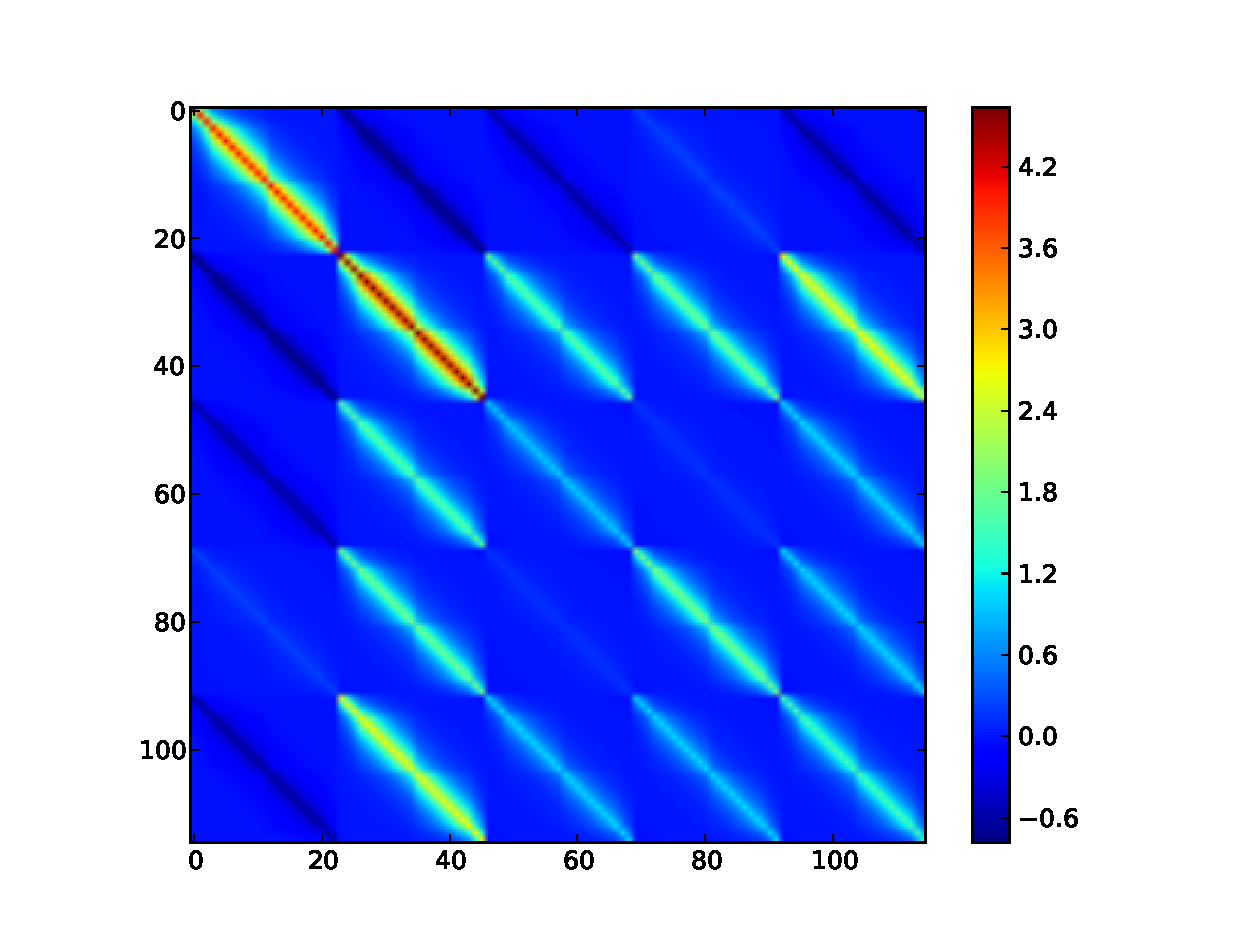
\includegraphics[width=0.5\textwidth,keepaspectratio]{diagrams/kern_6TF.eps}
	\rule{25em}{0.5pt}
	\caption[Kernel of intrinsic coregionalization model $\textbf{K}_f$ considering 5 transcription factors where covariance matrix $\boldsymbol{\Sigma}$ was constructed using Ornstein-Uhlenbeck kernel and White kernel in additive form] {Kernel of Intrinsic Coregionalization model $\textbf{K}_f$ considering five transcription factors (a random choice for better visualization) where covariance matrix $\boldsymbol{\Sigma}$ of $\left( Equation \ref{eq:K} \right)$ was constructed using Ornstein-Uhlenbeck kernel and White kernel in additive form.}
	\label{fig:kern_6TF}
\end{figure}
\begin{figure}[!htbp]
	\centering
	\includegraphics[width=0.5\textwidth,keepaspectratio]{diagrams/RBFWh9TF.png}
	\rule{25em}{0.5pt}
	\caption[Variation of activities of transcription factors with exponentiated quadratic kernel and white kernel in additive form] {Variation of activities of different transcription factors with exponentiated quadratic kernel and white kernel in additive form. A solid line represents a posterior mean, and shaded area represents the 95\% confidence interval for a specific transcription factor. Different colour shows the transcription factor activity of randomly picked transcription factors. Here we have noticed that for every transcription factors the activities are extremely smooth. In practical case this behaviour is hilgly unlikely. So, a combination of exponentiated quadratic kernel and white kernel in additive form is not a very good choice to infer the transcription factor activity.}
	\label{fig:TFA_with_RBFnWhKernel}
\end{figure}
Finally the posterior mean of the conditional distribution  is %of Equation \ref{eq:predicYq} %\ref{eq:predictionTFA} 
is
\begin{equation} \label{eq:prediction_MuF}
\boldsymbol{\mu}_F = 
\mathbf{K}_{t_\star,t} \otimes \boldsymbol{\Sigma} \mathbf{V} \boldsymbol{\Lambda}
\left[ \mathbf{K}_{t,t} \otimes \boldsymbol{\Lambda} \mathbf{V}^T\boldsymbol{\Sigma} \mathbf{V} \boldsymbol{\Lambda} + \sigma^2 \mathbf{I} \right]^{-1}\mathbf{y}_q
\end{equation}
and the covariance of the conditional distribution is %of Equation \ref{eq:predicYq} given by
\begin{equation} \label{eq:prediction_CF}
\begin{split}
\boldsymbol{C}_F &= 
\mathbf{K}_{t_\star,t_\star} \otimes \boldsymbol{\Sigma} \\
& - \mathbf{K}_{t_\star,t} \otimes \boldsymbol{\Sigma}\mathbf{V} \boldsymbol{\Lambda}
\left[ \mathbf{K}_{t,t} \otimes \boldsymbol{\Lambda} \mathbf{V}^T\boldsymbol{\Sigma} \mathbf{V} \boldsymbol{\Lambda} + \sigma^2 \mathbf{I} \right]^{-1} \\
& \left[ \mathbf{K}_{t_\star,t} \otimes \boldsymbol{\Lambda} \mathbf{V}^T\boldsymbol{\Sigma}\right]
\end{split}
\end{equation}
Figure \ref{fig:kern_6TF} shows the pictorial representation of intrinsic coregionalization kernel (Equation \ref{eq:K}) $\textbf{K}_f$ considering 5 transcription factors where covariance matrix $\boldsymbol{\Sigma}$ of  was constructed using Ornstein-Uhlenbeck kernel and white kernel in additive form.
\begin{figure}[!htbp]
	\centering
	%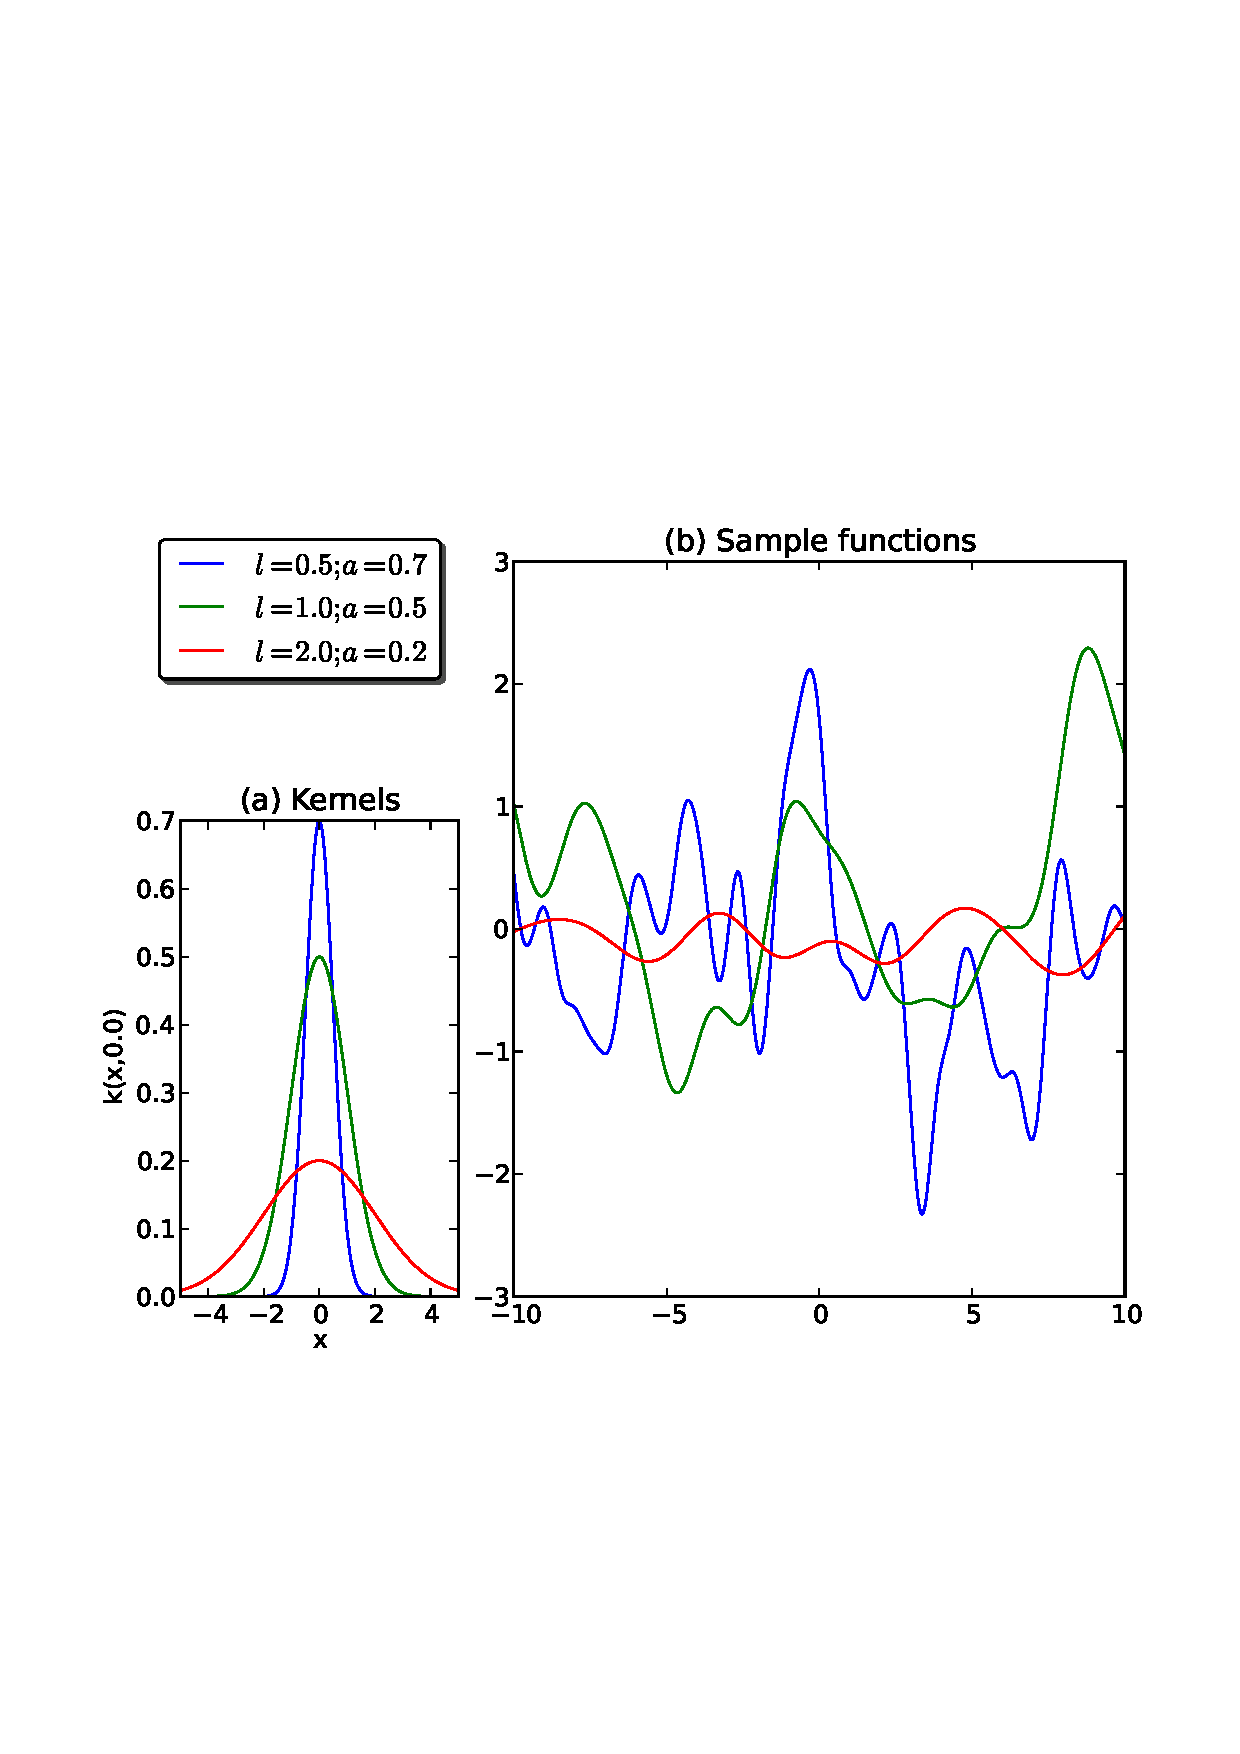
\includegraphics[width=10cm,keepaspectratio]{diagrams/SE_cov.pdf}
	\includegraphics[width=0.5\textwidth,keepaspectratio]{diagrams/ACE2_OU_Wh_9TF.png}
	\rule{25em}{0.5pt}
	\caption[Inference of transcription factor activity of ACE2]
	{Transcription factor activity of ACE2. The solid line represents a posterior mean of transcription factor activity, and shaded area represents 95\% confidence interval. $x$-axis represents the time, and $y$-axis represent the transcription factor activity. Here a \lq x\rq{ }represents a gene expression level. At any time point, multiple gene expression levels (\lq x\rq) represent the level of gene expression obtained from different genes which were regulated by transcription factor ACE2. We inferred the transcription factor activity considering all these expression levels.}
	\label{fig:TFA_of_of_ACE2}
\end{figure}


 The preliminary concepts of this methodology was presented in \cite{Rahman:2016} and a Jupyter Notebook demo using programming language \emph{python} is available at \cite{Muhammad:2014}.

\section{Dataset and Result analysis}
\begin{figure*}
	\centering
	\includegraphics[width=.95\textwidth,keepaspectratio]{diagrams/OU20TF2.png}
	\rule{50em}{0.5pt}
	\caption[Transcription factor activity of different transcription factor]{Transcription factor activity of different transcription factors: individual plots shows the activity of the transcription factor. Here, the solid line represents a posterior mean and shaded area represents the 95\% confidence interval. $x$-axis represents the time and $y$-axis represent the TFA.}
	\label{fig:TFA_of_20TF}
\end{figure*}

Here in this experiment we used the classic \cite{Spellman:1998} yeast cell cycle dataset. The cell division cycle gene \emph{cdc15} time series data has 23 time points. 

Exponentiated quadratic kernel also known as Radial basis function (RBF) kernel is very smooth kernel compared to Ornstein-Uhlenbeck kernel and perhaps is not a very good choice for the determination of actual transcription factors activities. Still, it can figure out the basic nature of the activities with over smoothness. Figure \ref{fig:TFA_with_RBFnWhKernel} shows activities of different transcription factors while the model was developed considering exponentiated quadratic kernel with White kernel in additive form.

Figure \ref{fig:TFA_of_of_ACE2} shows transcription factor activity of ACE2. While developing the model we chose \emph{Ornstein-Uhlenbeck} kernel and White kernel in additive form. In Figure \ref{fig:TFA_of_of_ACE2}, we noticed at any time point, multiple gene expression levels (represented by black \lq x\rq) were present, which shows the level of gene expression at that time point from different genes. A transcription factor can regulate multiple genes. To infer the activity of a transcription factor, we have to consider all these expressions. Here, we inferred the transcription factor activity of ACE2 considering all these expression levels. Earlier, we described how  Ornstein-Uhlenbeck kernel can be used to model the transcription factor activities. So, here we believe, the Ornstein-Uhlenbeck kernel will consider the basic nature of the transcription factors activity while White kernel will deal the noise associated the collected gene expression data.

Figure \ref{fig:TFA_of_20TF} shows transcription factor activity of different (arbitrarily chosen) transcription factors  where we used our newly developed model. Here, as a prior we used Ornstein-Uhlenbeck kernel and White kernel. In the plot, a solid line represents a posterior mean of transcription factors activity and shaded area represents the 95\% confidence interval.

\section{Conclusion}
 The choice of the covariance function is the central step in modelling with a Gaussian process. In this paper, we developed a covariance function suitable for modelling the dynamics of transcription factor activity. We also justified the rationale behind choosing the Ornstein-Uhlenbeck kernel to achieve the goal.  
 
 We showed that the linear Gaussian model proposed by \cite{Sanguinetti:2006} is equivalent to a Gaussian process with a particular covariance function. In this paper, we, therefore, build a transcription factor activity model straight from the Gaussian process perspective. For given gene expression profiles and a connectivity information between genes and transcription factors, here we designed a covariance function for reconstructing transcription factor activities and overcome the restrictive state dependencies of Markovian assumptions. In the beginning, we assumed that the joint process across all transcription factor activities and across all time points might have some correlation, hence we introduced an intrinsic model of coregionalization for the joint process. We also introduced a mathematical formalism, based on a judicious application of singular value decomposition, to enable us to efficiently fit the Gaussian process in a reduced \lq transcription factor activity\rq{ }space. Finally, we prepared a \emph{jupyter notebook} and made it available online.\\ \ \\
%\textbf{\Large{Information Sharing Statement}}
%The tools proposed in the article are available on request from \url{https://sites.google.com/site/muftimahmud}.

%\noindent \textbf{Conflict of Interest Statement}: The authors declare that the research was conducted in the absence of any commercial or financial relationships that could be construed as a potential conflict of interest.
%\\
\textbf{Authors and Contributors}: This work was carried out in close collaboration
between both of the co-authors. NDL preliminarily defined the research theme. MAR
contributed an early design of the system and implemented it. NDL
refined the system development. MAR wrote the manuscript and NLD edited it. Both of the authors have contributed to, seen and approved the final manuscript.
%\\
%\textbf{Ethical Approval}: All procedures performed in studies involving human participants were in accordance with the ethical standards of the institutional and/or national research committee and with the 1964 Helsinki declaration and its later amendments or comparable ethical standards.
%\\
%\textbf{Informed Consent}: Informed consent was obtained from all individual participants included in the study.

%\begin{thebibliography}{99.}
%\bibitem{Lebedev2006} Lebedev MA, Nicolelis MA. Brain-machine interfaces: past, present and future. Trends Neurosci. 2006;29(9):537-46.
%\end{thebibliography}


\bibliographystyle{ieeetr} % use this to have URLs listed in References

\bibliography{references} % Path to your

%% BibTeX users please use one of
%\bibliographystyle{spbasic}      % basic style, author-year citations
%%\bibliographystyle{spmpsci}      % mathematics and physical sciences
%%\bibliographystyle{spphys}       % APS-like style for physics
%\bibliography{}   % name your BibTeX data base
%\bibliography{/home/muhammad/Dropbox/thesisCorrection/References/references}
\balance
\end{document}
%
%
%
%
%
%
%
%
%
%
%
%
%\begin{abstract}
%Insert your abstract here. Include keywords, PACS and mathematical
%subject classification numbers as needed.
%\keywords{First keyword \and Second keyword \and More}
%% \PACS{PACS code1 \and PACS code2 \and more}
%% \subclass{MSC code1 \and MSC code2 \and more}
%\end{abstract}
%
%\end{document}
%\section{Introduction}
%\label{intro}
%Your text comes here. Separate text sections with
%\section{Section title}
%\label{sec:1}
%Text with citations \cite{RefB} and \cite{RefJ}.
%\subsection{Subsection title}
%\label{sec:2}
%as required. Don't forget to give each section
%and subsection a unique label (see Sect.~\ref{sec:1}).
%\paragraph{Paragraph headings} Use paragraph headings as needed.
%\begin{equation}
%a^2+b^2=c^2
%\end{equation}
%
%% For one-column wide figures use
%\begin{figure}
%% Use the relevant command to insert your figure file.
%% For example, with the graphicx package use
%  %\includegraphics{example.eps}
%% figure caption is below the figure
%\caption{Please write your figure caption here}
%\label{fig:1}       % Give a unique label
%\end{figure}
%%
%% For two-column wide figures use
%\begin{figure*}
%% Use the relevant command to insert your figure file.
%% For example, with the graphicx package use
%  %\includegraphics[width=0.75\textwidth]{example.eps}
%% figure caption is below the figure
%\caption{Please write your figure caption here}
%\label{fig:2}       % Give a unique label
%\end{figure*}
%%
%% For tables use
%\begin{table}
%% table caption is above the table
%\caption{Please write your table caption here}
%\label{tab:1}       % Give a unique label
%% For LaTeX tables use
%\begin{tabular}{lll}
%\hline\noalign{\smallskip}
%first & second & third  \\
%\noalign{\smallskip}\hline\noalign{\smallskip}
%number & number & number \\
%number & number & number \\
%\noalign{\smallskip}\hline
%\end{tabular}
%\end{table}
%
%
%%\begin{acknowledgements}
%%If you'd like to thank anyone, place your comments here
%%and remove the percent signs.
%%\end{acknowledgements}
%
%% BibTeX users please use one of
%%\bibliographystyle{spbasic}      % basic style, author-year citations
%%\bibliographystyle{spmpsci}      % mathematics and physical sciences
%%\bibliographystyle{spphys}       % APS-like style for physics
%%\bibliography{}   % name your BibTeX data base
%
%% Non-BibTeX users please use
%\begin{thebibliography}{}
%%
%% and use \bibitem to create references. Consult the Instructions
%% for authors for reference list style.
%%
%\bibitem{RefJ}
%% Format for Journal Reference
%Author, Article title, Journal, Volume, page numbers (year)
%% Format for books
%\bibitem{RefB}
%Author, Book title, page numbers. Publisher, place (year)
%% etc
%\end{thebibliography}
%
%\end{document}
% end of file template.tex
